\documentclass[a4paper]{article}
\usepackage{german}
\usepackage[utf8]{inputenc}

\usepackage{pgfplots}
\usepackage{pgfplots.assert}

\usepgfplotslibrary{fillbetween}

\begin{document}
\thispagestyle{empty}
\parindent=0pt
\parskip10pt

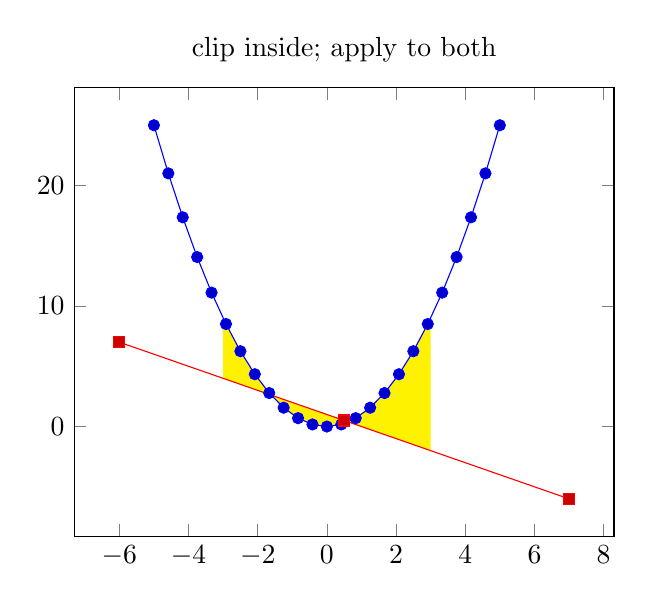
\begin{tikzpicture}
	\begin{axis}[title={clip inside; apply to both}]
	\addplot+[name path=A] {x^2};

	\addplot+[name path=B,domain=-6:7,samples=3] {1-x};

	\path[name path=clip];

	\addplot[yellow] fill between[of=A and B,
		soft clip={(axis cs:-3,-5) rectangle (axis cs:3,40)},
	];
	\end{axis}
\end{tikzpicture}

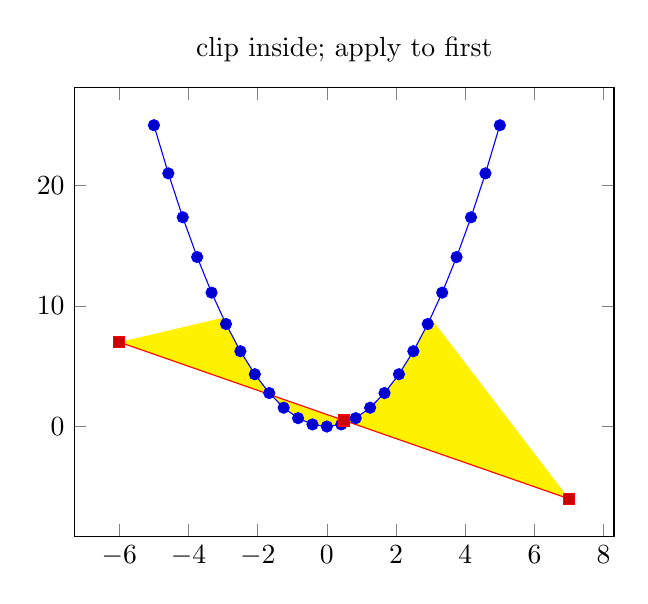
\begin{tikzpicture}
	\begin{axis}[title={clip inside; apply to first}]
	\addplot+[name path=A] {x^2};

	\addplot+[name path=B,domain=-6:7,samples=3] {1-x};

	\path[name path=clip];

	\addplot[yellow] fill between[of=A and B,
		soft clip first={(axis cs:-3,-5) rectangle (axis cs:3,40)},
	];
	\end{axis}
\end{tikzpicture}
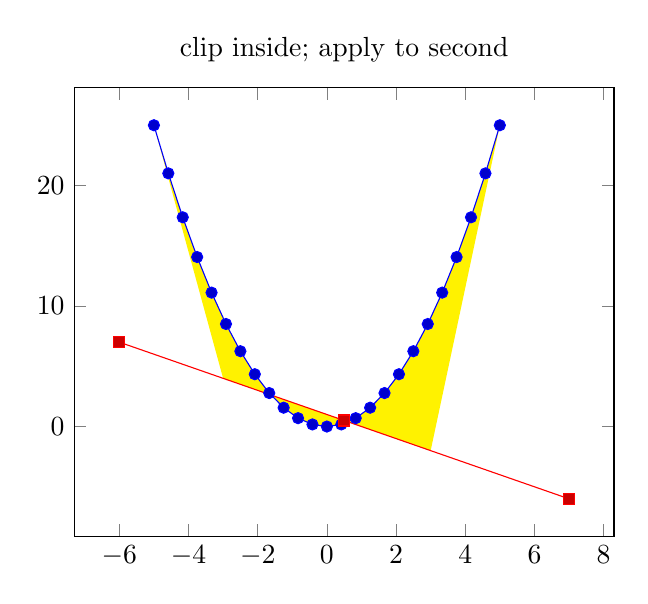
\begin{tikzpicture}
	\begin{axis}[title={clip inside; apply to second}]
	\addplot+[name path=A] {x^2};

	\addplot+[name path=B,domain=-6:7,samples=3] {1-x};

	\path[name path=clip];

	\addplot[yellow] fill between[of=A and B,
		soft clip second={(axis cs:-3,-5) rectangle (axis cs:3,40)},
	];
	\end{axis}
\end{tikzpicture}

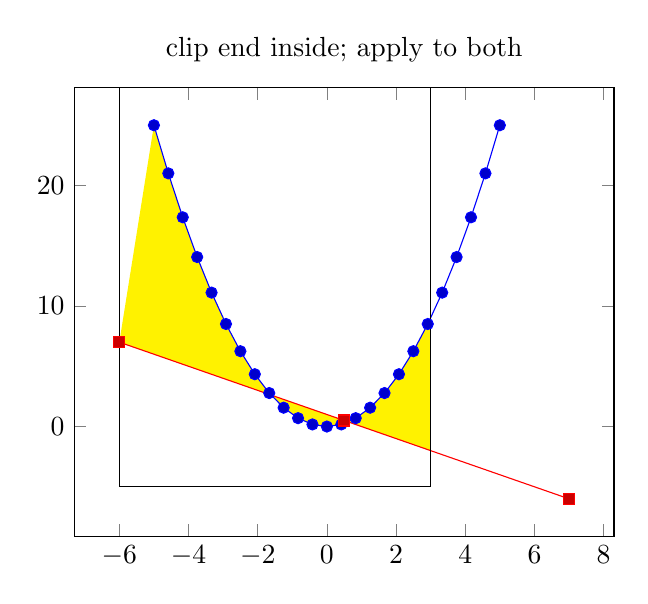
\begin{tikzpicture}
	\begin{axis}[title={clip end inside; apply to both}]
	\addplot+[name path=A] {x^2};

	\addplot+[name path=B,domain=-6:7,samples=3] {1-x};

	\path[name path=clip];

	\draw (axis cs:-6,-5) rectangle (axis cs:3,40);
	\addplot[yellow] fill between[of=A and B,
		soft clip={(axis cs:-6,-5) rectangle (axis cs:3,40)},
	];
	\end{axis}
\end{tikzpicture}
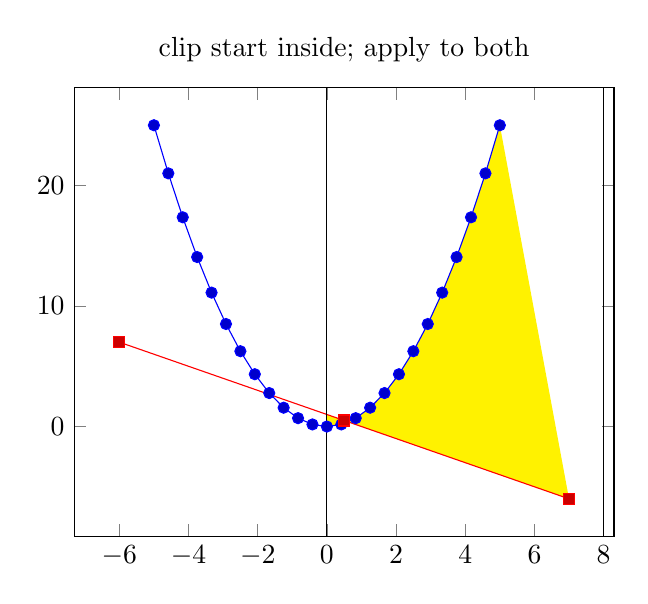
\begin{tikzpicture}
	\begin{axis}[title={clip start inside; apply to both}]
	\addplot+[name path=A] {x^2};

	\addplot+[name path=B,domain=-6:7,samples=3] {1-x};

	\path[name path=clip];

	\draw (axis cs:0,-10) rectangle (axis cs:8,40);
	\addplot[yellow] fill between[of=A and B,
		soft clip={(axis cs:0,-10) rectangle (axis cs:8,40)},
	];
	\end{axis}
\end{tikzpicture}


\end{document}

